\subsection{Game}

\subsubsection{Introduction}
The game implemented is {\it The Scorched Land Defense} as described in the compendium. The game has
to players playing concurrently. Player A is a Tank starting in the lower left corner. The tanks
mission is to get to the upper right corner before it gets shot by the cannon. The cannon is
controller by Player B. Its objective is to shot the cannon before it gets to its corner. The cannon
can use the Scorched land defence tactic by blowing up land in the field. The tank cannot drive
where the cannon has shot.

Each player has 4 lifes and the game ends when one player is defated 4 times.

\subsubsection{How to play}

\begin{figure}[h]
  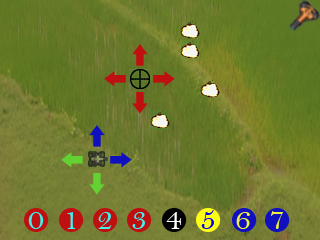
\includegraphics[width=350px]{graphics/buttons_illustration.jpg}

\end{figure}

Player A uses button 1-3 and Player B has buttons 4-8. Player A has two modes which it uses button 3
to toggle between. It can use buttons 1 and 2 to either move North and East or South and West.

Player B uses button 8, 7, 6 and 5 to move its aim left, down, up and right. It shots it cannon on
the field where its aiming currently with button 4.

\subsubsection{Design}

The /game folder contains the objects used in the game. The most importaint is the {\bf Controller}
which handles the communication between the modules in the game. The {\bf Cannon}, {\bf Tank} and
{\bf Field} are models for the objects in the game. The {\bf Button} and {\bf Led} objects are
wrapper object around the char drivers, to make communication easier.

\begin{figure}[h]
  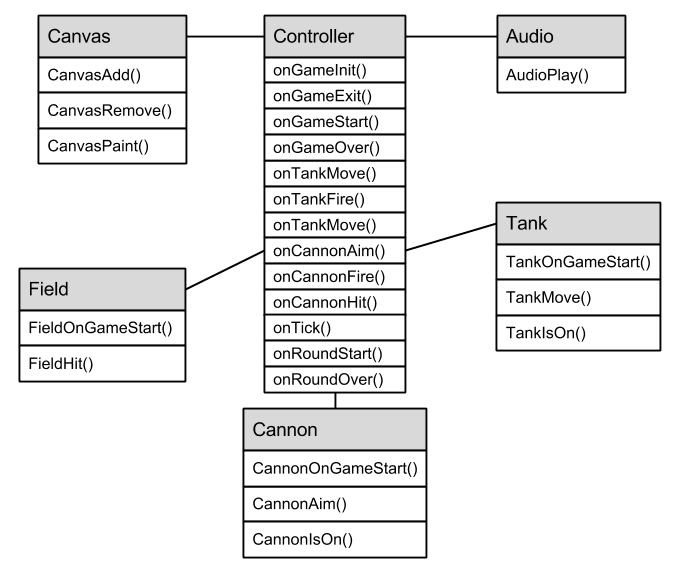
\includegraphics[width=350px]{graphics/game_UML.png}
\end{figure}
